\chapter{System Design}
\label{sec:design}

\section{System Components}
As shown in Figure~\ref{fig:sieve}, Sieve
consists of three components: a user client,
a storage provider daemon, and an import
daemon run by third party web
services. The \textbf{Sieve client} runs
on each user device. The client implements
a Javascript library which allows users to define the
access policies for each web service
(\S\ref{sec:policies}). For each policy, the
client generates the associated ABE
decryption key, and sends it to the
appropriate web service. Before the user
uploads an object to the storage provider,
the Sieve client transparently signs the
object with a per-user RSA key, and then
encrypts the object and signature with the
relevant ABE attributes (\S\ref{sec:attrGen}).
To protect against lost or stolen devices,
the RSA signing key and the ABE master secret
are partitioned across user devices; before a
client can sign or encrypt an object, the
client must participate in a secret sharing
protocol with two-factor authentication
(\S\ref{sec:secretSharing}).

The \textbf{storage provider daemon}
accepts encrypted data from Sieve clients.
Each encrypted object is tagged with
cleartext attributes. The storage provider
builds an index of these attributes so
that, when a web service requests objects
with attributes $a_0,\ldots,a_N$, the
storage provider can efficiently locate
those objects (\S\ref{sec:attrGen}).

The \textbf{Sieve import daemon} is run
by a third party web service. The import
daemon accepts ABE keys and upload
notifications from Sieve clients. After
receiving an upload notification, the import
daemon fetches encrypted objects from the
storage provider. The import daemon then
decrypts the objects using its ABE key,
and feeds the cleartext data into the
web service's legacy pipeline for consuming
user data (\S\ref{sec:attrGen}).

From the perspective of a third party,
a user's Sieve storage is read-only;
only the user can write
new objects and update old ones. Third
parties use their own storage for data
that is derived from a user's Sieve
objects.

\section{Usage Model}

In theory, any web service that imports
user data is compatible with Sieve. In
practice, certain kinds of web services
and user data are easier to integrate into
the Sieve model. Sieve works best with
  \begin{smitemize}
    \item data streams that are tightly
          bound to a particular user, and
    \item web services that can tolerate
          those data streams being read-only
          (and perhaps only partially disclosed).
  \end{smitemize}
Examples of Sieve-amenable data streams
include demographic information like age and
location; sensitive financial and medical
records; sensor data from quantified self
applications; longitudinal, cross-site
histories of browsing behavior and e-commerce
transactions; and multimedia data streams
containing photos, videos, and audio.
Examples of web services that consume such
data streams are social media applications
like Instagram~\cite{instagram}, 
exercise trackers like Open mHealth~\cite{omh}, 
and financial analysis sites like Mint~\cite{mint}
that require access to a user's spending habits.

Applications like Reddit~\cite{reddit} 
and StackOverflow~\cite{soverflow} are
less appropriate for Sieve. In these applications,
user data has less standalone value to the
owner; instead, most of the value derives from
embedding the data in a larger, service-specific
context like a Reddit discussion.
%@@@Cut the text paragraph below is crunched for space.
Web-based email is also an awkward fit for the
Sieve model, since email services require mutable,
per-user state like mailboxes, but Sieve exports
read-only storage. An email service could pull
read-only outgoing messages from Sieve storage,
and implement the mutable mailbox state on the
service's own machines. However, such an
architecture would be awkward, since users
would have no way to selectively expose
\emph{incoming} messages to the mail service.

\section{Overview of ABE}
\label{sec:abeOverview}

\begin{figure}
  \centering
     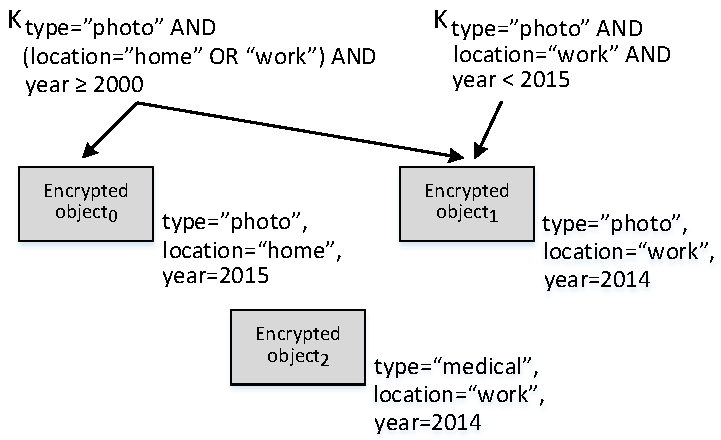
\includegraphics{figs/abeExample.pdf}
     \caption[ABE Example]{In this example, there are two ABE keys at the
              top, and three ABE-encrypted objects at the bottom.
              An arrow indicates that a key can decrypt a particular
              object.}
  \label{fig:abeExample}
\end{figure}

In attribute-based encryption~\cite{kpabe}, a
cleartext object is associated with attributes
that govern how the object is encrypted. Each
decryption key has an access control structure
(ACS) which enumerates one or more attributes.
An ACS can test an attribute for equality (e.g.,
\texttt{location=``Paris''}) or comparative
value (e.g., \texttt{age > 35}). An ACS can
also chain those simple tests using \texttt{ANDs},
\texttt{ORs}, and \texttt{NOTs}. As shown in
Figure~\ref{fig:abeExample}, a key can only decrypt
an object if the key's ACS matches the object's
attribute values.

We use the shorthand notation $K_{a_0,\ldots,a_N}$
to refer to an ABE key whose ACS contains the
attribute tests $a_0,\ldots,a_N$. All tests are
implictly joined via \texttt{ANDs} unless we
explicitly note otherwise.

\section{Assigning Attributes to User Data}
\label{sec:attrGen}

Raw user data comes from a variety of
sources. Some of it is directly generated
by a user's devices; for example, a user
might enter financial information directly into a
spreadsheet. Data might also come from an
external source, like an email attachment.
Sieve associates each object, regardless
of its provenance, with a set of attributes.

Some attributes can be automatically assigned
by hardware, like the GPS coordinates for a
running route. Other attributes can be
extracted by software, using application-specific
transducers or semantic file systems~\cite{sfs,contextsfs,graphsfs}.
Users can also manually tag objects. Sieve is
agnostic to the manner in which attributes
are assigned, although our implementation of
the Sieve client provides a GUI which simplifies
manual tag assignment.

Users and web services must agree on data schemas,
so that web services can meaningfully aggregate
and process information from different users. In
particular, web services need to know a
standardized set of attributes which are defined
by user data. To define this standardized set,
Sieve uses FOAF~\cite{FOAF} as the schema % http://xmlns.com/foaf/spec/   [For higher-level overview, see http://en.wikipedia.org/wiki/FOAF_%28ontology%29]
model for data about human users, and RDF~\cite{RDF} %http://www.w3.org/TR/2014/REC-rdf11-concepts-20140225/  [For higher-level overview, see http://en.wikipedia.org/wiki/Resource_Description_Framework]
as the schema model for data about user objects.

Each Sieve user has a standardized FOAF record
which stores basic scalar information like
her name, location, and birthday. Sieve
associates each entry in the FOAF record
with an ABE attribute; for example, a user's
name is associated with the $userName$ attribute.
Sieve does not upload the actual FOAF record
to the storage provider, since the only purpose
of the FOAF record is to standardize the
metadata that is associated with each user.
Instead, Sieve uploads individual FOAF
entries, encrypting each one with the associated
ABE attribute (e.g., $<alice>_{K_{userName}}$,
such that the user's name can only be
decrypted by web services whose ABE keys
possess the $userName$ attribute).

Sieve associates each data object with a
type-specific RDF schema. For example, a
W2 tax record has attributes for the user's
pre-tax income, her number of dependents,
and so on. Similar to FOAF records, RDF
records are only used to define a standard
attribute set for each data type. Sieve uploads 
individual encrypted RDF entries (e.g., $<2>_{K_{numDependents}}$)
to the storage provider.

Some data objects like images are not
decomposable, i.e., each object is disclosed
or not disclosed at the granularity of the
entire object. For objects like this, Sieve
uploads the entire object, encrypting it
using the standardized RDF attributes and
any manually added user tags. For example,
a photo has standard attributes like height
and width, and may also possess user-defined
tags like ``Vacation'' or ``Family.''

As applications evolve, RDF and FOAF schemas
may change. Sieve is compatible with
preexisting techniques for synchronizing
schema changes across a distributed system~\cite{f1,maintaindataware, onthefly}.

\section{Uploading Data to the Storage Provider}
\label{sec:dataPush}

Suppose that the user wishes to upload a file
$F$ that has attributes $a_0,\ldots,a_N$.
Before uploading the file, the Sieve client
must encrypt the file such that decryption
is only possible with the ABE key whose ACS
match the attributes $a_0,\ldots,a_N$. The na{\"i}ve
approach is to directly encrypt $F$ with
$K_{a_0,\ldots,a_N}$. However, ABE is a form of
public key cryptography, and it is significantly
slower than symmetric key cryptography. Thus,
Sieve uses a \textit{hybrid encryption} scheme,
encrypting the file data with a symmetric key,
and encrypting the symmetric key with ABE.

The end-to-end upload protocol is the following.
First, Sieve generates a symmetric AES key $k$,
and uses that key to encrypt $F$. Sieve uploads
the encrypted $<F>_k$ to the storage provider.
The storage provider responds with a GUID for
the file. Sieve then uploads a \emph{metadata
block} for $F$. The metadata block is an encrypted
pointer containing $<GUID, k>_{K_{a_0,\ldots,a_N}}$.
Only principals which possess keys with ACSes that
match $a_0,\ldots,a_N$ can
decrypt the pointer, fetch the object, and
decrypt the object.

In the next section, we describe how web services
acquire ABE keys. For now, we merely say that
users do not share ABE keys with storage providers.
Thus, a storage provider cannot inspect the data
that it stores. The provider can try to tamper
with the data or produce fake user data, but
Sieve clients sign each object with a user-specific
RSA key before encrypting the object and its signature, 
allowing web services to detect tampering.

From the perspective of a third party
web service, Sieve storage is read-only.
However, a user is free to create new
objects, delete old ones, and update
objects that reside at preexisting
GUIDs. If a user's device has cached
the GUID and the symmetric key for a
particular object, the user can update
that object directly, without having
to fetch the associated metadata block
and incur ABE overheads to decrypt it.

\section{Defining and Enforcing Access Policies}
\label{sec:policies}

In Sieve, all user data is private by
default, since users must explicitly
share ABE decryption keys that provide
access to data. When a third party requests
access permissions, e.g., upon the first
time that a user visits a site, the user
generates an access policy for the site.
Policies are defined in terms of attributes,
and the Sieve client provides a GUI which
makes it easy for users to explore which
attributes her data contains, and which
objects would be exposed for a given policy.
Policies are simple boolean expressions;
for example, a web service used by a
physician might receive the policy
(fileType=``medicalRecord''
AND year>2010 AND doctor=``John'').

After the user has defined a policy, her
Sieve client assembles the ABE master secret
(\S\ref{sec:secretSharing}) and generates
an ABE key with the appropriate ACS. The
Sieve client then sends the key and the name
of the user's storage provider to the remote
web service. The message is protected with SSL/TLS~\cite{tls}
to ensure confidentiality and integrity.
Later, when the web service desires to
access user data, the service does not
need to interact with the user. Instead,
the service sends an access request directly
to the
user's storage provider. The request
contains a list of the attributes which
belong to the data of interest. The
storage provider returns the encrypted
metadata blocks for the relevant objects.
The web service decrypts the metadata,
revealing the GUIDs for the requested
objects as well as their symmetric
encryption keys. The web service uses the
GUIDs to fetch the encrypted objects.
After decrypting the objects locally,
the service feeds the cleartext data
into an application-specific data pipeline.

Once that happens, Sieve is uninvolved in
the application workflow. Thus, Sieve is
compatible with the current web ecosystem
which uses third party computation and
storage to add value to user data. However,
Sieve provides users with cryptographically
strong control over the raw data that each
service receives. Sieve's access policies
also have three attractive properties:
  \begin{smitemize}
    \item The number of policies (and keys) scales with
          the number of web services that a user
          shares with, not the much larger number
          of objects that she owns.
    \item Policy generation is decoupled from
          object generation. At object creation
          time, users do not have to speculate
          a priori about whom a new object might
          be shared with.
    \item Policies safeguard objects using
          cryptography, but users are insulated
          from the details of key management.
  \end{smitemize}
Given all of this, we believe that Sieve
strikes a good balance between security,
usability, and backwards compatibility with
current web services.


\section{Key Revocation}
\label{sec:revocation}

In Sieve, an individual object is encrypted
with a symmetric key $k$; the object's metadata
block (which contains $k$ and the object's
GUID) is encrypted with an ABE key $K_{a_0,\ldots,a_N}$.
A web service caches its ABE key, and it may also
cache symmetric keys and GUIDs, to avoid
repeated fetches and decryptions of metadata
blocks. Caching makes revocation tricky,
since a user that wants to revoke a service's
access rights cannot force the service to delete
cached keys. An honest storage provider can
refuse access requests from deprivileged third
parties, but if the storage provider is
compromised, it can leak data that is
encrypted with ostensibly revoked keys
that are still in the wild.

To protect against storage server compromise,
Sieve revokes keys by \emph{re-encrypting}
user data and metadata with new keys that
are not shared with the newly deprivileged
third party. If the storage provider is
honest at the time of rekeying, then even
if it is compromised later, it will never
leak data that is encrypted with revoked
keys.
%!!!jwm: That's almost true; there is some
%        subtlety involving the synchronization
%        protocol for the counters. If a device
%        is late in hearing the latest counter
%        increment, there will be a period of
%        time during which it will upload data
%        using the old counter value. So, we
%        might need to tweak the phrasing of
%        the last sentence in the paragraph
%        above.
Leveraging homomorphic encryption~\cite{gentry},
the storage provider re-encrypts the data
locally, using a rekeying token provided
by the user. The storage provider learns
nothing about the old encryption key, the
new encryption key, or the underlying cleartext;
the user avoids the need to download, re-encrypt, and 
re-upload data from her personal devices.

In the rest of this section, we first describe
how data is re-encrypted, and then explain how
the metadata is re-encrypted.

\subsection{Re-encrypting data} Up to this point, 
we have assumed that Sieve 
encrypts data using a standard
symmetric cipher like AES 
(\S\ref{sec:dataPush}). However, to enable storage
providers to re-encrypt data in situ, Sieve
must instead employ a key homomorphic pseudorandom
function~\cite{keyhom, npr99}. We
define that function $F$ as
  \begin{equation*}
    F(k, x) = H(x)^k 
  \end{equation*}
where $H$ is a hash function and $k$ is the
secret key associated with each object. $F$
is additively key homomorphic, which means
that, for two keys $k$ and $k'$,
$F(k,x)*F(k',x) = F(k+k',x)$.

Using $F$, we define an encryption scheme whose
security and performance are similar to those
of AES. Like AES-CTR, our new encryption scheme
operates on blocks of data, and uses a random
counter to convert a block cipher into a stream
cipher. In our new scheme, the $j$th ciphertext
block $c_j$ is equal to
  \begin{equation*}
    c_j = m_j \cdot F(k, N + j)
    \label{new_enc}
  \end{equation*}
where $m_j$ is the $j$th cleartext block, and
$N$ is a public nonce that is equivalent to the
initialization vector in AES-CTR. To decrypt,
a third party extracts $k$ from a metadata
block and performs the 
following calculation:
  \begin{equation*}
    m_j = c_j \cdot F(-k, N + j)
  \end{equation*}
To revoke the ABE key $K_{a_0,\ldots,a_N}$, a user's
Sieve client generates a \emph{rekeying token}
for each object that is accessible via
$K_{a_0,\ldots,a_N}$. For an object encrypted by
$k$, the rekeying token is $\delta = -k + k'$,
where $k'$ represents the new encryption key
for the object. The client sends $\delta$ to
the storage provider; this operation is safe
because the provider cannot recover $k$ or $k'$ 
from $\delta$. The storage provider
uses $\delta$ to compute a new version of
each ciphertext block $c_j$:
\begin{align*}
    c_{j,new} &= c_j \cdot F(\delta , N + j) \\
    &= m_j \cdot F(k, N+j) \cdot F(-k + k', N+j) \\
    &= m_j \cdot F(k', N+j)
\end{align*}
In this manner, the storage provider re-encrypts
objects without learning the encryption keys
or the underlying cleartext.

\subsection{Re-encrypting metadata} Each user
device maintains an integer counter called the
epoch counter. It is initialized to zero, and
represents the number of revocations that the
user has performed. When a user device
generates a new ABE key, Sieve automatically
tags the key with an $epoch$ attribute that
is set to the current value of the epoch
counter. The epoch attribute is a standard
ABE attribute; until now, we have elided the
$epoch$ attribute in key descriptions, but
we explicitly represent it in this section.

Suppose that a web service possesses the ABE
key $K_{a_0,\ldots,a_N,epoch=i}$, where $i$ is a
whole number. To remove the service's access
permissions, the user first re-encrypts the
affected data using homomorphic encryption.
The user then increments the epoch counter to
$i+1$. Next, the user generates a new metadata
block for each re-encrypted object, inserting
the new $k$. The user encrypts the new metadata
block and uploads it to the storage provider;
the metadata is encrypted using the updated
ABE key $K_{a_0,\ldots,a_N,epoch=i+1}$. Finally, the
user sends the new ABE key to any non-revoked
web services who possess the old version of
the key from epoch $i$; remember that if the
user gives multiple web services access to
$a_0,\ldots,a_N$, those services will receive
the same ABE key.

Additional web services may require new ABE
keys, depending on how the attributes in ABE
keys overlap. For example, consider two web services:
the first possesses \allowbreak $K_{(a_0\; OR\; a_1)\; AND\; epoch=0}$,
and the second has $K_{(a_1\; OR\; a_2)\; AND\; epoch=0}$.
Both keys grant access to a metadata block
with attributes $a_1\; AND\; epoch=0$. To revoke
the first key, Sieve re-encrypts the metadata
block using the attributes $a_1\; AND\; epoch=1$.
As a result, the second, non-revoked web service
loses access to the block. Thus, Sieve must
give an updated key $K_{(a_1\; OR\; a_2)\; AND\; epoch=1}$
to the second service.

When Sieve re-encrypts a data object, the
object's GUID stays the same, but its symmetric
key changes. This invalidates any cached keys
that are held by web services. So, when a
service receives an updated ABE key, the
service discards any cached symmetric keys
that were decrypted using the old version
of the ABE key. The signature is unaffected
because the signature is on the cleartext data, which
remains unmodified.

% !!!jwm: Note to self: This detail should go somewhere
%         else; it doesn't directly deal with revocation.
% Another small detail is that the user only
% stores the attributes it has assigned to web
% services to figure out what keys to reissue
% but not the corresponding ABE decryption key
% as a way to keep minimal sensitive information.

\subsection{Additional details} A Sieve user
will often possess multiple devices; for example,
a single user might possess a smartphone, a tablet, a
laptop, and a quantified life device like a
Fitbit. If a user has multiple devices, then
the device which initiates a revocation will
broadcast the revoked key and the new epoch
counter to the other devices. This ensures
that the other devices do not use an old epoch
number to encrypt new metadata blocks. Network
partitions may delay the rate at which devices
learn about the revocation, so when a device
receives a revocation notice, it proactively
rekeys any data and metadata that it mistakenly
encrypted using the revoked key. Computationally
weak devices like Fitbits can delegate rekeying
work to more powerful devices like laptops.

Revocation messages are signed by the public
key of the device that issued the message.
Devices learn about each other's public keys
at Sieve initialization time, and later, when
the user adds a new device. By signing revocation
messages, Sieve prevents arbitrary devices
from injecting fradulent revocation notices.

%!!!jwm: Make sure that we mention this point
%        in the intro.
To the best of our knowledge, Sieve is the
first ABE system which supports full re-keying
of \emph{both} data and metadata. Prior ABE systems either
cannot revoke keys at all~\cite{privio}, or can
only revoke access to metadata~\cite{persona,aauth,catchet};
in the latter case, data remains encrypted with
revoked symmetric keys, leaving that data vulnerable
to storage server compromise or negligence.


\section{Protecting Against Device Loss}
\label{sec:secretSharing}

At initialization time, Sieve creates an ABE
master secret. Sieve uses the master secret
to derive the ABE decryption keys that are
given to web services. Thus, the entire
cryptosystem is compromised if the master
secret is lost.

In a straightforward implementation of ABE, each
user device has a copy of the master secret.
However, portable devices like smartphones and
tablets are often lost~\cite{wang2012smartphone},
meaning that a na\"{\i}ve implementation of ABE
exposes the master secret to great risk. Even if
users encrypt the master secret with a
password-derived key~\cite{pbkdf}, users often
pick weak passwords~\cite{gaw2006password},
giving the master secret weak protection in
practice if a device is lost.

To mitigate the impact of lost devices, Sieve
uses Shamir secret sharing~\cite{shamir} to
partition the master secret across a user's
devices. In a $(k,n)$ sharing scheme, the
secret is divided across $n$ devices, and
$k$ shares are required to reconstruct the
secret. In the context of Sieve, this means
that when a user device needs to generate
an ABE key, the device must first gather $k-1$
shares from other devices. Only then can the
device assemble the master secret, generate
the ABE decryption key, send the key to the
web service, and then delete the local copy
of the assembled master secret.

When the master secret is being assembled,
Sieve requires the user to explicitly authorize
each participating device to release its local
share. By default, Sieve uses a $k$ of 2, so
this authorization scheme is similar to
two-factor authentication~\cite{twofactor}---a user
cannot generate an ABE decryption key unless
she controls two separate devices (e.g., a
laptop and a smartphone). This means that,
if an attacker finds a single lost device,
that device cannot generate the master secret.

Sieve also employs secret sharing to protect
the user's signature key. During uploads to
the storage provider, the signature key is
used to authenticate the client-side of the
SSL/TLS session. Thus, the storage provider
can reject fradulent upload attempts from
arbitrary devices.

Secret sharing protects the ABE master secret
and the user's signing key. However, a lost
device possesses a device key that is used to
authenticate messages from that device. An
attacker with a lost device can try to use
the device key to subvert the revocation
protocol (\S\ref{sec:revocation}). For example,
if a malicious lost device can roll back the
epoch to a \emph{smaller} number, uncompromised
devices will upload new data that can be
decrypted with revoked keys. To prevent attacks
like this, Sieve relies on the multi-factor
authentication that is built into the secret
sharing protocol---revocation requires a device
to assemble the master secret, and assembling
the master secret requires the user to possess
multiple devices.

%@@@Delete is crunched for space.
To add or remove devices from the secret sharing 
scheme, or to change $k$, the user must invalidate
the old shares. To do so, the user must find $k$
devices to participate in a new secret sharing
exchange that uses the updated $k$ and $n$.
% This process invalidates the old shares
% on any lost devices as long as only $k-1$
% devices are lost before resetting the shares.

Sieve provides no protections against a subverted
device that the user believes is not lost or
malfunctioning. For example, if the user wants
to upload data from the smartphone that she
is currently using, and the smartphone has a
rootkit, the phone can arbitrarily delete the
user's data, upload garbage, or improperly
revoke keys.

\section{Minimizing ABE Overheads}
\label{sec:minAbeCost}

Until now, we have assumed that clients
perform two encryptions for every object
upload: an ABE encryption for the metadata
block, and a symmetric encryption for
the data block. ABE is a public key
cryptosystem, so ABE operations are an
order of magnitutude slower than symmetric
ones. Fortunately, Sieve clients can use
several techniques to reduce the frequency
of ABE operations.

The simplest approach is for clients to
store multiple objects inside each data block.
Creating the associated metadata block
will still require an ABE encryption,
but subsequent writes and reads of the data
block will only incur symmetric cryptography
costs---clients can update the data block
in-place, without changing the metadata,
and third parties can cache the data block's
symmetric key to use during reads. For
example, a smartphone with a GPS unit might
use a single data block to store a month's
worth of location data. The phone appends
new location samples to the current month's
data block, creating a new data block and
metadata block when a new month begins.

\begin{figure}
  \centering
     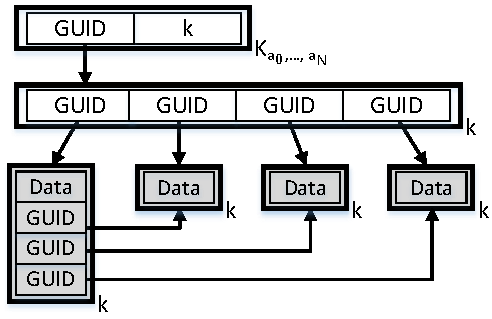
\includegraphics{figs/guidMap2.pdf}
     \caption[Example of Sieve storage-based data structure]
     {An example of a storage-based data structure. 
              Using indirect GUIDS, the metadata block at the top
              points to a data block that only contains GUIDS.
              Those GUIDs point to raw data blocks. Raw data blocks
              can also embed pointers, as demonstrated by the simple
              tree structure that links the data blocks.}
  \label{fig:guidMap}
\end{figure}

Clients can also leverage more complex \emph{storage-based
data structures}. For example, as shown in
Figure~\ref{fig:guidMap}, a Sieve client can
use indirect GUIDS like a Unix file system uses
indirect data pointers. In this scheme, the
top-level GUID for a storage-based data
structure refers to a metadata block that
points to a \emph{GUID map}. The GUID map
is just a data block that contains a symmetric
key and additional GUIDs; those GUIDs point to
raw data blocks that are encrypted with the
symmetric key. Once again, clients and web
services eliminate ABE costs by encrypting
many objects with the same symmetric key,
and caching that key.

Having many, smaller data blocks instead of
fewer, larger data blocks is useful if the
storage provider does not allow partial block
writes (meaning that all writes force the
client to upload at least a block's worth of
data).\footnote{For example, Amazon's S3
allows partial reads, but not partial writes~\cite{AmazonPUT}.} % http://docs.aws.amazon.com/AmazonS3/latest/API/RESTObjectPUT.html
For similar reasons, multiple small blocks
are useful if the symmetric cipher does
not allow new data writes or 
updates to random offsets in the
ciphertext.\footnote{Most commonly used 
block cipher modes, such as CBC and CTR mode,
do not easily support new writes to random offsets.}

A raw data block can also embed GUIDs which
reference other data blocks. This allows
a client to build more complex data structures
than flat arrays of data blocks.
More complex structures may be preferrable
if they can reduce the number of wide-area
data fetches that web services must perform.
For example, Figure~\ref{fig:guidMap} shows
a simple tree with a single parent and three
children; by convention, the parent of the
tree is the first entry in the GUID map. Each
data block can hold multiple items, but when
a block fills up, the client creates a new
data block, adds the associated GUID to
the GUID map, and then updates any internal
GUIDs within preexisting data blocks. A third
party whose ABE key decrypts the metadata block
can traverse the tree structure without
additional ABE operations, since all of the
data blocks are encrypted with the same
symmetric key. 

For future modifications to the data structure,
such as adding new or updating existing data
blocks or creating new pointers and GUIDs,
the user caches the relevant GUIDs and keys
(data and GUID map) allowing her to modify
the contents of the data structure without
creating a new metadata block, thus,
avoiding an ABE operation. Similarly, a web
service could and should cache the same information
and use it to download any changes to the data 
structure to avoid incurring the cost of ABE 
operation. However, the caching is acceptable
because the user can revoke the web service's
access to her un-accessed data using Sieve's
revocation protocol (\S\ref{sec:revocation})

Each storage-based data structure defines a
Python API for adding and removing objects,
as well as traversing the entire structure.
Sieve clients and web services cache the
metadata blocks for storage-based data
structures, and use the Python APIs to
interact with those structures. Thus, Sieve
clients and web services are insulated from
the low-level details of GUID maps (although
both parties can access raw storage if desired,
and if Sieve's ABE policies allow such accesses).

Sieve's revocation protocol
is compatible with GUID maps, which are re-encrypted
in place, just like any other data block. However,
when Sieve determines that a metadata block must
be re-keyed, Sieve checks whether the metadata
refers to a GUID map. If so, Sieve must chase
the GUIDs in the GUID map to identify the
raw data blocks that must be re-keyed. The revocation
protocol does not change the GUIDs that are
associated with re-keyed data blocks, so embedded
GUIDs inside data blocks remain valid after
re-keying.
% A user can also use the revocation protocol
% to revoke access for any lost or stolen device
% with cached keys and GUIDs similarly to the way
% that users revoke access for web services
% with cached GUIDs and keys.

Each data block that is referenced by
a particular GUID map is encrypted with the
same $k$. However, Sieve uses counter-mode
encryption~\cite{ctrmode}, and employs a
different counter for each block.
%\footnote{The counter is a public initialization
% value at the beginning of the ciphertext.}
Thus, if an attacker learns the cleartext
for one ciphertext block, the attacker does
not have an easier job of decrypting other
ciphertext blocks with the same $k$.

\section{Relabelling}
\label{sec:relabel}

In Sieve, a user may relabel an object. For
example, a user can restrict access by adding
an additional attribute to the object. A user
can also remove attributes, or swap one
attribute for another.

To implement relabelling, a user's Sieve
client performs three actions. First,
the client replaces the old
metadata block on the storage server with a new one 
that contains a new symmetric key 
and is ABE-encrypted using the new attributes.
Second, the client uses homomorphic encryption to
re-encrypt the object under the new symmetric key 
on the storage server.
Finally, the client updates storage-based
references to the object, ensuring that the
references adhere to the object's new access
policy. The client can locate these references
because the client knows the old attributes
for the object, the new attributes for the
object, and the attributes for all of the user's
metadata blocks. Thus, the client can determine
which references must be patched. For example,
suppose that a user has two storage-based data
structures $S_0$ and $S_1$; further suppose that,
due to relabelling, an object must move from
$S_0$ to $S_1$. By inspecting the object's old
attributes, the client determines that the object
was originally referenced by $S_0$. The client
homomorphically re-encrypts the object using
symmetric key $k'$, traverses $S_0$ to remove
any references to the object, and then adds a
$<GUID, k'>$ reference for the object to $S_1$.
Sieve performs the traversals, removals, and
additions using the APIs defined by the
storage-based data structures.

\section{Discussion}
\label{sec:discussion}

%@@@Cut if crunched for space.
\subsection{Alternative policy languages}
Attribute-based disclosure policies are easy
for users to understand, and these policies
naturally map to ABE cryptosystems. However,
ABE cannot express arbitrarily complex policy
functions. Garbled circuits~\cite{lindell2009proof}
and functional encryption~\cite{boneh2011functional}
are Turing complete, but they are prohibitively
slow. For example, garbled circuits decrypt
AES data at a rate that is four orders of
magnitude slower than native AES decryption~\cite{justGarble}.
Relative to functional encryption and garbled
circuits, ABE is several orders of magnitude
faster. We believe this trade-off is worthwhile.


\subsection{Paying for storage} 
In Sieve,
each user places her objects in private cloud
storage. Someone must pay for that storage.
One option is for ad networks to pay. In Sieve,
ad networks can be third parties, and they can
receive ABE keys to access user data. Using a
micropayment system like FileTeller~\cite{fileteller},
advertisers could pay for the right to collect
longitudinal data about a user, and generate
targeted advertisements based on that data.
By deferring user storage costs, advertisers
would encourage users to continue to declassify
a subset of their data. Indeed, since each user
now stores all of her data in a single place
instead of multiple locations, ad networks
would gain access to more contextual information
than in the web ecosystem, even if users choose
which objects to reveal~\cite{adnostic}. Thus,
Sieve might enable a happy middle ground in
which users gain explicit control over the data
seen by third parties, and third parties willingly
subsidize private user storage in return for
better contextual information.

If ad-driven storage subsidies are poorly
designed, they may lead to perverse trade-offs
between subsidy amounts and the required
levels of data disclosure. A full study of
such interactions is beyond the scope of
this paper. For now, we merely observe that
some users may opt out of the subsidy system
entirely. These users will have to pay for
their own storage, but there is reason to
believe that they would do so. Well-known
sites like Pandora, Slashdot, and OkCupid
already allow users to pay a small monthly
fee to remove advertisements, so there is a
preexisting demographic which is willing to
pay money in exchange for better privacy.
The popularity of open source applications
also demonstrates that developers are willing
to make high quality applications without the
expectation of direct payments from users.
Thus, we believe that Sieve's application
model is realistic.

\subsection{Efficient data importing} 
In the
current web ecosystem, users explicitly submit
data to web services, making it easy for those
services to determine when new information
has been created. In Sieve, users submit new
data to the storage provider. However, user
devices know the tags that are associated
with both new data items and web service ABE
keys; thus, when a device uploads an object
of interest to a particular service, the device
can proactively notify the service of the upload.

Storage-based data structures (\S\ref{sec:minAbeCost})
also make it easy for services to identify new
data. For example, using a storage-based log,
user devices can append new data to the head of
the log. A service can cache the GUID and the
symmetric key for the log head, and periodically
check the beginning of the log for new objects.

\subsection{Anonymity across services} 
Some users may not want to be tracked across
different web services. For example, a user
might be comfortable sharing data with services
$X$ and $Y$, but uncomfortable with $X$ knowing
how she interacts with $Y$, and vice versa.
Sieve cannot restrict what services do once
they possess user data, so Sieve cannot prevent
$X$ and $Y$ from pooling their data and trying
to correlate user behavior across both services.
Users can employ various techniques to make
tracking more difficult. For example, proxies
like Tor~\cite{tor} allow users to hide their
IP addresses from web services. However, users can also
establish a unique login identity for each web
service, or lobby web services to use anonymous
credential systems~\cite{camenisch2001efficient}. 
Unfortunately, Tor and anonymous credential
systems rely on network proxies that hurt
application responsiveness, and seemingly
anonymized data sets can still reveal sensitive
user information to machine learning algorithms~\cite{dwork2011differential}.
Thus, providing anonymity on the web is still
an important area for future research.

\section{Implementation}
\label{sec:implementation}
Our Sieve prototype consists of a Sieve
client, a storage provider daemon, and a
Sieve import daemon that is run by third
parties. Each component is written in Python,
and uses PyCrypto~\cite{pyCrypto} to implement
RSA and AES. For ABE operations, we use the
libfenc~\cite{libfenc} library with elliptic
curves~\cite{mnt224} from the Stanford
Pairing-Based Cryptography library~\cite{pbc}.
To build Sieve's key homomorphic symmetric
cipher~\cite{keyhom}, we use the Ed448-Goldilocks
elliptic curve library~\cite{ed448}.

The storage provider daemon uses BerkeleyDB~\cite{berkdb}
to store encrypted data blocks, and MongoDB~\cite{mongodb}
to store metadata blocks. For each data block,
the key is a GUID, and the value is a symmetrically
encrypted object. For a metadata block, the
key is a set of cleartext ABE attributes, and
the value is an ABE-encrypted GUID and symmetric
key. Metadata blocks are indexed by their
attribute fields, and all metadata blocks for
a particular user are stored in a MongoDB
collection.
% The libfenc library and Ed448-Goldilocks
% elliptic curve libraries are written in C++,
% so whenever we use these libraries,
% we make RPC calls from our Python
% code to call these functions.

The JavaScript code in a web site interacts
with the local Sieve client using a small
RPC library that we provide. When a web site
initially requests access to a user's data,
the site's JavaScript sends an \texttt{XMLHttpRequest} 
to a localhost webserver run by the Sieve
client. The Sieve client then displays a
GUI that allows the user to define an
access policy for the site, and send the
associated ABE key to the site's web server.

